\documentclass[8pt, a4paper]{article}
 
\usepackage{amsfonts, amsmath, amssymb}
\usepackage[utf8]{inputenc}
\usepackage[russian]{babel}
\usepackage[dvips]{graphicx}
\usepackage{listings}
 
\begin{document}

\author{Дмитрий Кондрашкин}
\title{Отчет к задаче: ``Применение метода ближайшего соседа, решение реальной задачи''}
\maketitle

Обучающая выборка состоит из $107000$ объектов. Объекты разделены на два класса. Имеется
9 признаков. Задача состоит в классификации объекта.

При визуализации признаков можно заметить большое количество шума(например рис.~\ref{feat3} и рис.~\ref{feat8}).
С помощью этих графиков выборка была вручную очищена от шумов. Было удалено около 4000 объектов.
Затем данные были отнормированны на отрезок $[0,1]$.

Для решения задачи использовался метод $k$ ближайших соседей.

Был произведен выбор оптимального $k$, для различных метрик: $l_2$, $l_1$, $l_{\propto}$.
Перебирались значения $k=1 \hdots 20$. Для каждого $k$ алгоритм три раза запускался на случайных подвыборках
размера $N=20000$. Результаты усреднялись. График зависимости качества $AUC$ от $k$ приведен на
рис.~\ref{metrics}.
В результате эксперимента было выбрано оптимальное значение $k=12$, и $l_1$ метрика.
При этих параметрах $AUC=69.68\%$.
\begin{figure*}[h]
    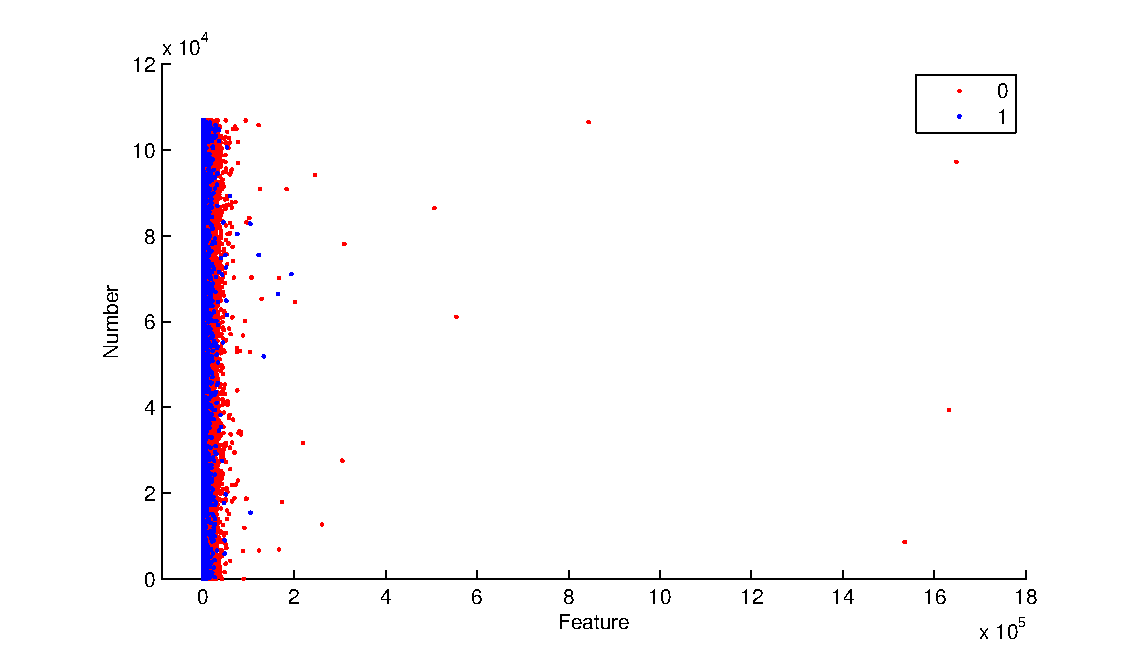
\includegraphics[width=\textwidth]{feat3.eps}
    \caption{Шумы в признаке 3}
    \label{feat3}
\end{figure*}
\begin{figure*}[h]
    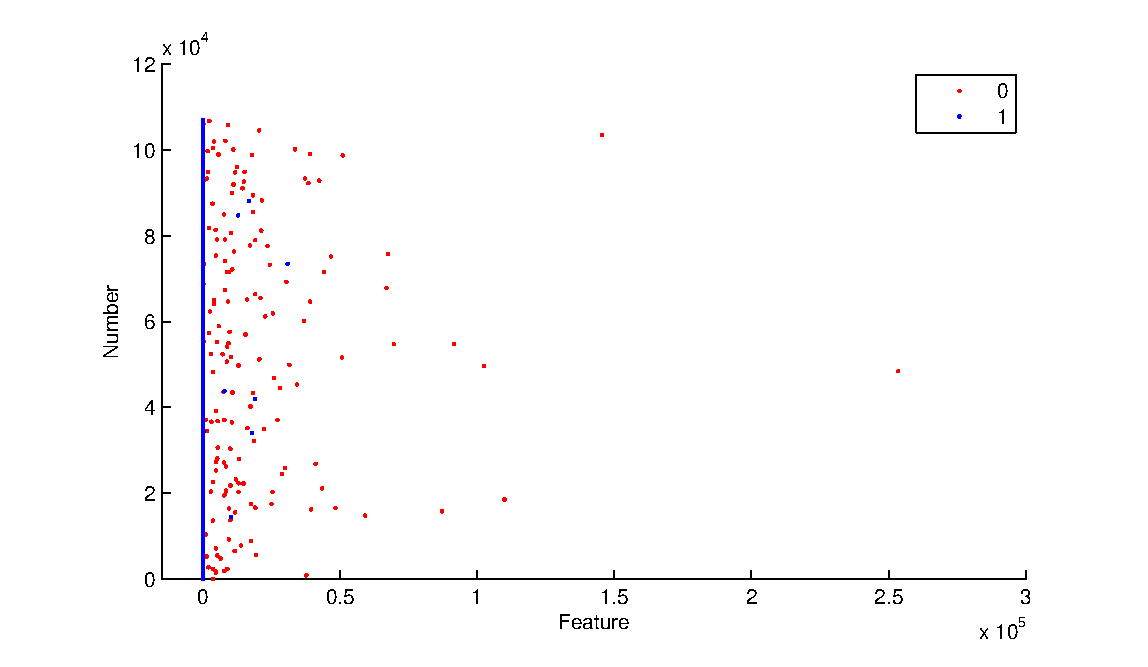
\includegraphics[width=\textwidth]{feat8.eps}
    \caption{Шумы в признаке 8}
    \label{feat8}
\end{figure*}
\begin{figure*}[h]
    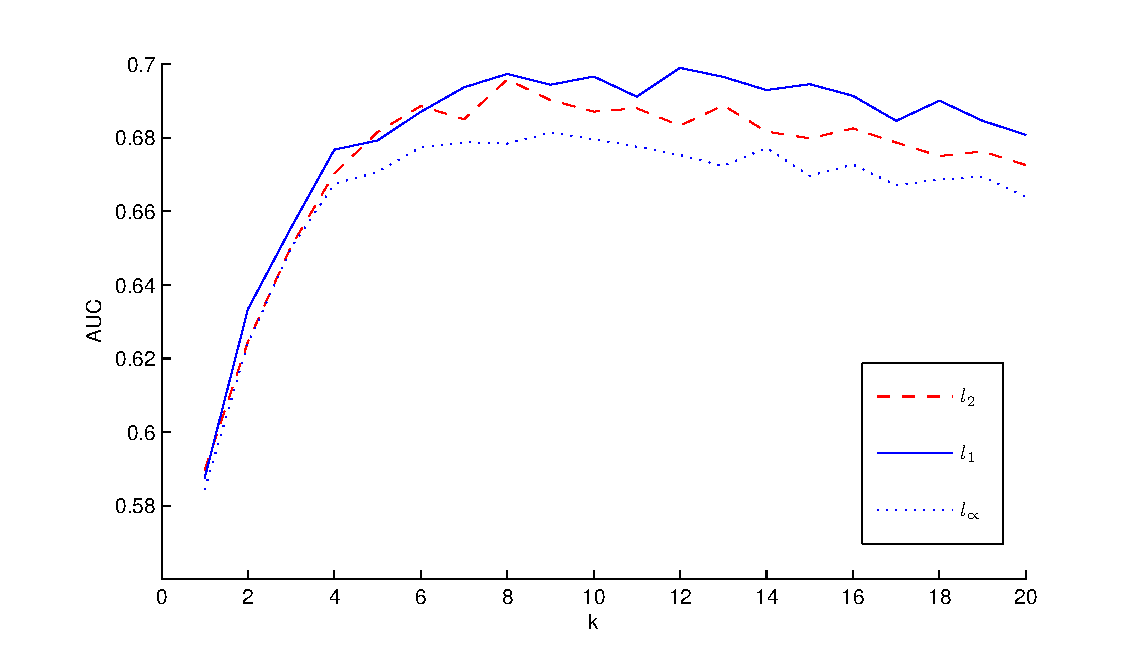
\includegraphics[width=\textwidth]{metrics.eps}
    \caption{Зависимость качества от $k$ для различных метрик}
    \label{metrics}
\end{figure*}

\end{document}
